\section{Results}\label{sec:result}

Given an SPN symmetric-key primitive and the parameter $A$ indicating the maximum number of S-boxes to be considered, we first generate graph $G$ according to our method in Section \ref{sec:gen_G}. Applying our method in Section \ref{sec:find_ite_c}, we find the best iterative characteristic in $G$. Applying our method in Section \ref{sec:find_ite_h}, we find the best iterative distinguisher with rounds no moret than 5 and 10 resp. Applying our method in Section \ref{sec:method-edp-elp}, we find the best differential or linear hull containing iterative sub-characteristics. 

%Comparing the two results, we show the strength of the clustering effect through a bar chart. 

\subsection{Results on Finding Iterative Distinguishers}

We apply our methods to 6 SPN symmetric-key primitives including KNOT\cite{zhang2019knot}, RECTANGLE\cite{zhang2015rectangle}, PRESENT\cite{bogdanov2007present}, GIFT\cite{banik2017gift}, PUFFIN\cite{cheng2008puffin} and TRIFLE\cite{Datta2019trifle}. For each of the primitives, we first apply Algorithm \ref{algo:gen-g}/\ref{algo:gen-g-equiv} in order to generate the interesting graph. Then we apply Algorithm \ref{algo:find-ite-c}/\ref{algo:find-ite-c-equiv} in order to finding the best single iterative characteristic. However, by considering the clustering effect, we may find better iterative distinguishers. We apply Algorithm \ref{algo:find-ite-h}/\ref{algo:find-ite-h-equiv} in order to find the best iterative differential or linear hull with rounds no more than 5 and 10 respectively. 

The results on differential iterative distinguishers are shown in Table \ref{tab:ite-ddt} while the results on linear iterative distinguishers are shown in Table \ref{tab:ite-lat2}. 
%The results on differential iterative distinguishers are shown in Figure \ref{fig:bar_ddt} while the results on linear iterative distinguishers are shown in \ref{fig:bar_lat2}. The height of a blue bar is the best average weight growth of a single iterative characteristic. The height of an orange bar is the best average weight growth of an iterative differential or linear hull with rounds no more than 5. The height of a green bar is the best average weight growth of an iterative differential or linear hull with rounds no more than. According to the two figures, linear characteristics in most cases have a stronger clustering effect than differential characteristics. 

We show the generated graphs for KNOT and RECTANGLE in Figure \ref{fig:graph-rect-ddt}, \ref{fig:graph-rect-lat2}, \ref{fig:graph-knot256-ddt}, \ref{fig:graph-knot256-lat2} and the generated graph containing linear iterative characteristics in Figure \ref{fig:graph-gift64-lat2} for GIFT-64. The detailed edges of the generated graphs are shown in Table \ref{tab:dis-rect-ddt}, \ref{tab:dis-rect-lat2} and \ref{tab:dis-gift64-lat2}. The red parts of a generated graph are its strong components. The rest parts of a generated graph are marked with blue. We can see that they are one-way paths linking two different strong components. 

In the following, we show some additional results for some of the primitives. 

%The results on differential cryptanalysis are shown in Figure \ref{fig:bar_ddt} and those on linear cryptanalysis are shown in Figure \ref{fig:bar_lat2}. Applying our algorithm in Section \ref{sec:find_ite_c}, we obtain the weight growth of the best iterative characteristic which are shown as the blue bars. Applying our algorithm in Section \ref{sec:find_ite_h} given $r$, we obtain the weight growth of the best $r$-round iterative distinguisher. Allowing an iterative distinguisher of too many rounds is meaningless, for in practice an iterative distinguisher is used to construct a long-round distinguisher. Thus we obtain the minimum weight growth of the best iterative distinguisher with $r\leq 5$ as shown in the orange bars and $r\leq 10$ as shown in the green bars. 
\begin{table}
	\caption{Results on differential iterative distinguishers}\label{tab:ite-ddt}
	\centering
	\begin{tabular}{|c||c|c||c|c||c|c|}
		\hline
		cipher & $A$ & \tiny$\min\limits_{r,u\in G}-\log_2c(p_{u,u})/r$ & $A$ & \tiny$\min\limits_{r\leq 5,u\in G}-\log_2c(h^r_{u,u})/r$ & $A$ & \tiny$\min\limits_{r\leq 10,u\in G}-\log_2c(h^r_{u,u})/r$ \\
		\hline
		KNOT-256 & 2 & 5.33 & 3 & 5.33 & 3 & 5.18 \\
		\hline
		RECTANGLE & 2 & 5.00 & 3 & 5.00 & 3 & 5.00 \\
		\hline
		GIFT-64 & 2 & 5.00 & 3 & 5.00 & 3 & 4.93 \\
		\hline
		PRESENT & 2 & 4.50 & 3 & 4.42 & 3 & 4.21 \\
		\hline
		TRIFLE-BC & 1 & 3.00 & 2 & 3.00 & 2 & 3.00 \\
		\hline
		PUFFIN & 1 & 2.00 & 2 & 1.95 & 2 & 1.91 \\
		\hline
	\end{tabular}
\end{table}

\begin{table}
	\caption{Results on linear iterative distinguishers}\label{tab:ite-lat2}
	\centering
	\begin{tabular}{|c||c|c||c|c||c|c|}
		\hline
		cipher & $A$ & \tiny$\min\limits_{r,u\in G}-\log_2c(p_{u,u})/r$ & $A$ & \tiny$\min\limits_{r\leq 5,u\in G}-\log_2c(h^r_{u,u})/r$ & $A$ & \tiny$\min\limits_{r\leq 10,u\in G}-\log_2c(h^r_{u,u})/r$ \\
		\hline
		KNOT-256 & 2 & 6.00 & 3 & 5.46 & 3 & 5.15 \\
		\hline
		RECTANGLE & 2 & 6.00 & 3 & 5.70 & 3 & 5.46 \\
		\hline
		GIFT-64 & 2 & 6.00 & 3 & 6.00 & 3 & 6.00 \\
		\hline
		PRESENT & 1 & 4.00 & 1 & 3.37 & 1 & 2.96 \\
		\hline
		TRIFLE-BC & 1 & 4.00 & 1 & 3.54 & 1 & 3.09 \\
		\hline
		PUFFIN & 1 & 2.00 & 1 & 1.86 & 1 & 1.81 \\
		\hline
	\end{tabular}
\end{table}

%\begin{figure}
%    \centering
%    \caption{Results on differential iterative distinguishers for some SPN block ciphers including KNOT-256, RECTANGLE, PRESENT, GIFT-64, PUFFIN and TRIFLE. The y-axis is the smallest negative logarithm of the differential probability of a differential iterative distinguisher. The height of a blue bar is the best average weight growth of a single differential iterative characteristic. The height of an orange bar is the best average weight growth of an $r$-round iterative differential with $r\leq 5$. The height of a green bar is is the best average weight growth of an $r$-round iterative differential with $r\leq 10$. }
%	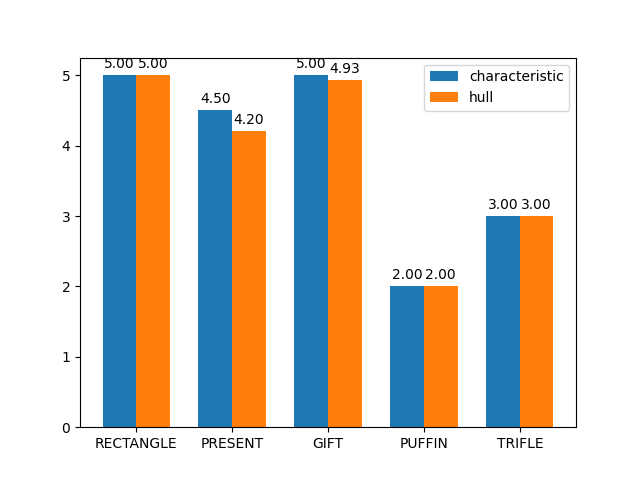
\includegraphics[width=1\textwidth]{fig/bar_ddt.png}
%	\label{fig:bar_ddt}
%\end{figure}

%\begin{figure}
%    \centering
%    \caption{Results on linear iterative distinguishers for some SPN block ciphers including KNOT-256, RECTANGLE, PRESENT, GIFT-64, PUFFIN and TRIFLE. The y-axis is the smallest negative logarithm of the linear correlation square of a linear iterative distinguisher. The height of a blue bar is the best average weight growth of a single linear iterative characteristic. The height of an orange bar is the best average weight growth of an $r$-round iterative linear hull with $r\leq 5$. The height of a green bar is is the best average weight growth of an $r$-round iterative linear hull with $r\leq 10$. }
%	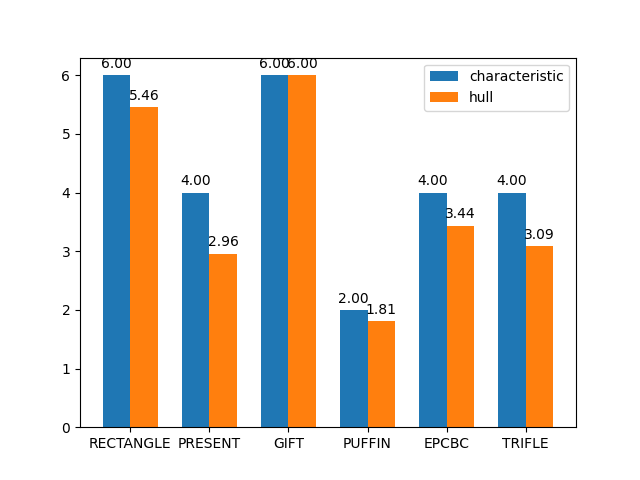
\includegraphics[width=1\textwidth]{fig/bar_lat2.png}
%	\label{fig:bar_lat2}
%\end{figure}

%In the following, we list the experimental settings and results for each of the ciphers. 
%Comparing the two figures, we find that linear iterative distinguishers have stronger clustering effect than differential ones. For each seperate primitives, we list the experimental settings and analysis of results. 

%\subsubsection{RECTANGLE \cite{zhang2015rectangle}} The state of RECTANGLE is treated in two dimensions. Each column is a 4-bit S-box which can be implemented using a bit-slice technique. Left rotational shifts are conducted on each of the 4 rows in parallel. The two operations of RECTANGLE has the rotational symmetry and thus we search for its rotational iterative characteristics. By setting $A=2$, the best differential rotational iterative characteristic we found is a 1-round one with input difference $x_0=0x2,x_5=0x6$, output difference $x_15=0x2,x_4=0x6$ and probability $2^{-5}$. By setting $A=3$, we can't find better rotational iterative differentials. By setting $A=2$, we found two best linear rotational iterative characteristics with average weight growth $6$. By setting $A=3$, the average weight growth of the best linear distinguisher we found is $5.46$ which is better than that obtained by only considering single linear characteristics. 

%\subsubsection{KNOT \cite{zhang2019knot}} KNOT is a round 2 candidate of the NIST lightweight cryptography standardization process. Its inner permutations are inheritors of RECTANGLE, also utilizing components with rotational symmetry. The primary version of it uses a 256-bit inner permutation. By setting $A=2$, we find its best differential and linear iterative characteristics. By setting $A=3$, we find stronger iterative distinguishers. 

%We set $A=3$ in both cases of differential and linear cryptanalysis. We find that the linear characteristics has clustering effect. But we note that the weight growth of the best iterative differential and linear distinguishers are equal, implying that its securities against differential and linear cryptanalysis are balanced. 

\subsubsection{PRESENT} The only best differential characteristic we find is exactly the one given in \cite{wang2008differential}. In \cite{ohkuma2009weak}, the author gives the construction of 1-bit linear characteristics. Our results are in compliance with the work in \cite{ohkuma2009weak} that the 1-bit linear characteristics have strong clustering effect. Note that the 1-S-box linear characteristics are 1-bit linear characteristic due to that the bit permutation spread the 4 output bits of 1 S-box to 4 input bits of 4 different S-boxes in the next round. 

\subsubsection{GIFT-64} From Table \ref{tab:ite-lat2}, it's shown that all primitives have clustering effect on linear characteristics except GIFT-64. To explore the reason, we draw the graph containing linear iterative characteristics in Figure \ref{fig:graph-gift64-lat2}. It's shown that the four iterative characteristics have no common masks. 

%\subsubsection{PUFFIN \cite{cheng2008puffin}} We set $A=1$ to find its best iterative characteristic. It has both comparatively weak securities against differential and linear cryptanalysis.

%\subsubsection{EPCBC \cite{yap2011epcbc}} We set $A=1$ in the linear case. We can't find any iterative differential characteristic though $A$ is set up to 3. But it has comparatively weak security against linear cryptanalysis. 

\subsubsection{TRIFLE} In \cite{liu2019iterative}, a 1-round differential characteristic is found using MILP method. It's also found using our method. Another best differential iterative characteristic we find has 127 rounds. 

\subsubsection{GIFT-128 \cite{banik2017gift}} We test out method on GIFT-128. We find no differential and linear characteristics even though $A$ is set up to 3. It's interesting that how to design a primitive with no low-weight iterative characteristic using a bit permutation as its linear layer. 

\subsubsection{ASCON \cite{dobraunig2016ascon}} We also test our method on the inner permutation of ASCON. We find no differential and linear characteristics even though $A$ is set up to 3. 
%attributed to its strong diffusion linear layer. 

%\begin{figure}\label{fig:plot_ite}
%    \centering
%    \caption{Results on some SPN block ciphers, which are RECTANGLE, PRESENT, GIFT64, PUFFIN, EPCBC and TRIFLE from top to bottom resp. For each subfigure, the x-axis is the number of rounds. For a subfigure in the left column, the y-axis is the weight of differential probability, while for a subfigure in the right column, the y-axis is the weight of correlation square. The red spot denotes the best single iterative characteristic with fewest rounds obtained by Algo. \ref{algo:find_ite_c_G}. The yellow (green, blue) line denotes the best iterative hull with $A=$1 (2, 3).} 
%	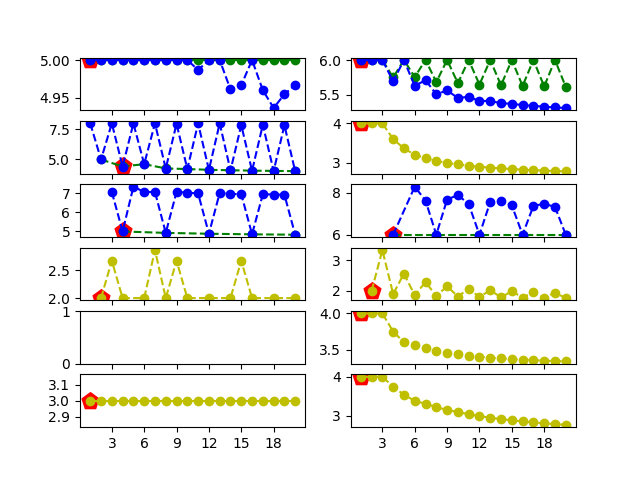
\includegraphics[width=1\textwidth]{fig/iterative.png}
%\end{figure}


\begin{figure}[htbp]
	\centering
	\caption{The generated graphs for RECTANGLE and KNOT256.}
	\subfigure[RECTANGLE, differential, $A=2$]{
	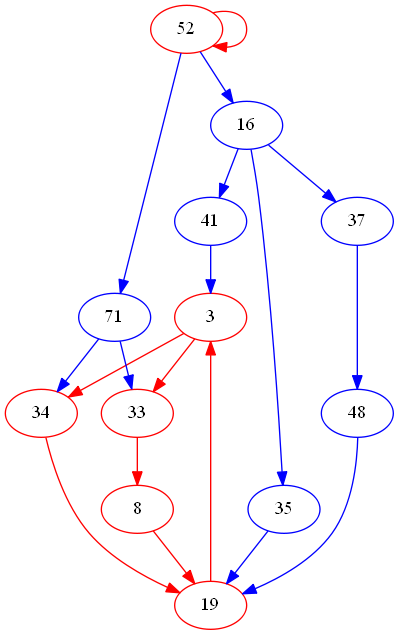
\includegraphics[width=5.5cm]{fig/graph_rect_ddt.png}
	\label{fig:graph-rect-ddt}
	}
	\quad
	\subfigure[RECTANGLE, linear, $A=2$]{
	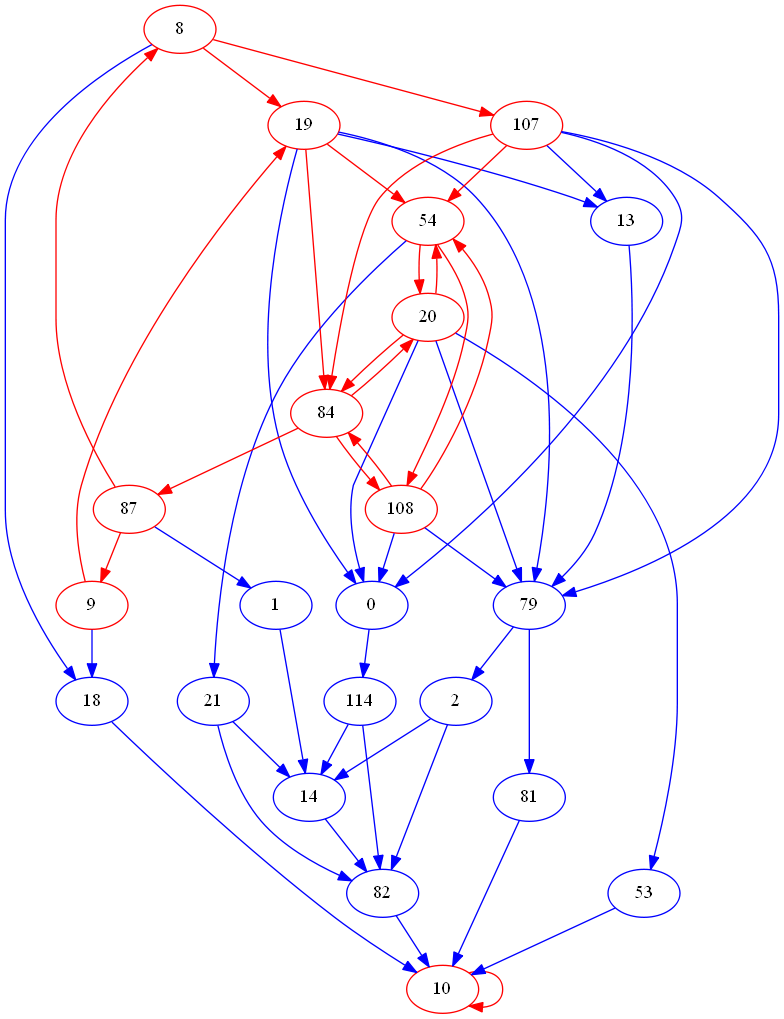
\includegraphics[width=5.5cm]{fig/graph_rect_lat2.png}
	\label{fig:graph-rect-lat2}
	}
	\quad
	\subfigure[KNOT256, differential, $A=2$]{
	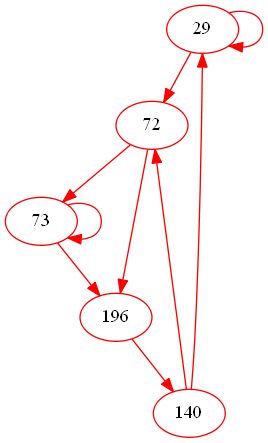
\includegraphics[width=4.5cm]{fig/graph_knot256_ddt.png}
	\label{fig:graph-knot256-ddt}
	}
	\quad
	\subfigure[KNOT256, linear, $A=2$]{
	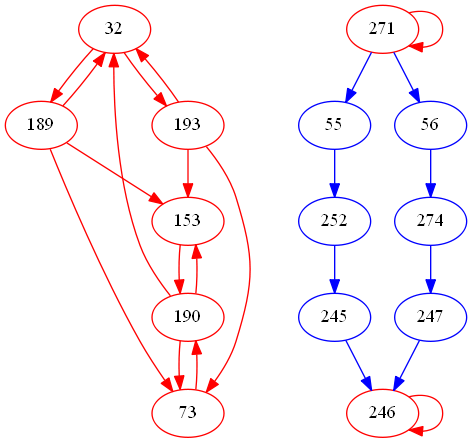
\includegraphics[width=6.5cm]{fig/graph_knot256_lat2.png}
	\label{fig:graph-knot256-lat2}
	}
\end{figure}

\begin{figure}
    \centering
	\caption{The generated graph containing linear iteractive characteristics for GIFT-64 when $A=2$}
	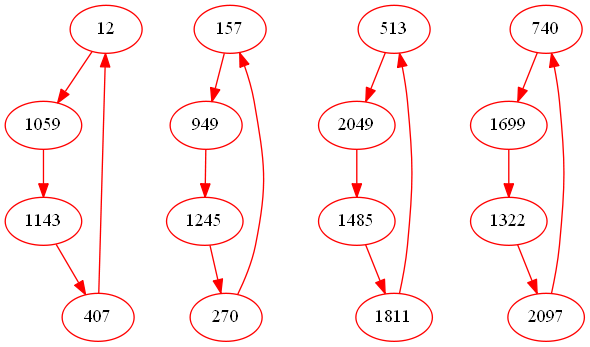
\includegraphics[width=0.8\textwidth]{fig/graph_gift64_lat2.png}
	\label{fig:graph-gift64-lat2}
\end{figure}

\subsection{Results on Finding the Best Differentials and Linear Hulls Containing Iterative Sub-characteristics}

We apply our Algorithm \ref{algo:msg}/\ref{algo:msg-equiv} to the 6 SPN primitives: KNOT-256, RECTANGLE, PRESENT, GIFT-64, PUFFIN and TRIFLE-BC. The results are given in Table \ref{tab:EDP} and Table \ref{tab:ELP}. 

For PRESENT, GIFT-64 and RECTANGLE, the results are very close to those in \cite{EPRINT:HalVej18}. For PUFFIN, we find both better differential and linear distinguishers than \cite{EPRINT:HalVej18} did. For TRIFLE-BC, the best differential distinguisher we find is a little better than the single 43-round differential characteristic given in \cite{liu2019iterative}. And we find a 51-round linear distinguisher while TRIFLE-BC has full rounds of 50. For KNOT-256, the designers only gave the results on the best single characteristics: a 48-round exploitable differential one and a 44-round exploitable linear one \cite{zhang2019knot}. We find a 53-round exploitable differential and a 56-round exploitable linear hull, improving the designers' results by 5 and 12 rounds respectively. 

\begin{table}
	\caption{Results on finding the best differential containing iterative sub-characteristics. $r$ is the number of rounds. $A$ is the maximum number of active S-boxes a difference we consider can has. $(rb,wb)$ determines the scope of extended differential characteristics we consider. $-\log_2\max\limits_{u\in S_0,v\in S_r}c(p_{u,v})$ is the probability of the best differential characteristic we find. $-\log_2\max\limits_{u\in S_0,v\in S_r}c(h^r_{u,v})$ is the probability of the best differential we find. $T$ is the running time of the whole process}\label{tab:EDP}
	\centering
	\begin{tabular}{|c|c|c|c|c|c|c|}
		\hline
		cipher & $r$ & $A$ & $(rb,wb)$ & $-\log_2\max\limits_{u\in S_0,v\in S_r}c(p_{u,v})$ & $-\log_2\max\limits_{u\in S_0,v\in S_r}c(h^r_{u,v})$ & $T$(h) \\
		\hline
		%PRESENT & 15 & 3 & (4,14) & 66 & 58.02 & 8s+5753s\\
		%PRESENT & 16 & 2 & (3,10) & 70 & 62.13 & 0s+42s\\
		PRESENT & 16 & 3 & (3,10) & 70 & 61.81 & 0.0 \\
		\hline
		%GIFT-64 & 12 & 2 & (3,13) & 58 & 56.57 & 0s+40s\\
		GIFT-64 & 13 & 2 & (3,13) & 62 & 60.42 & 0.0\\
		\hline 
		RECTANGLE & 14 & 2 & (6,25) & 61 & 60.65 & 133 \\
		\hline
		%KNOT-256 & 52 & 2 & (3,12) & 274 & 251.83 & 0s+10s\\
		%KNOT-256 & 52 & 2 & (3,10) & 274 & 252.41 & 1s+359s\\
		%KNOT-256 & 52 & 2 & (3,12) & 274 & 252.26 & 1s+1054s\\
		%KNOT-256 & 52 & 3 & (3,12) & 274 & 249.20 & 6s+11342s\\
		KNOT-256 & 53 & 3 & (3,12) & 274 & 254.38 & 0.2 \\
		\hline
		PUFFIN & 32 & 2 & (2,7) & 64 & 58.43 & 0.6 \\
		\hline
		TRIFLE-BC & 43 & 2 & (2,7) & 127 & 126.35 & 1.0 \\
		\hline
	\end{tabular}
\end{table}

\begin{table}
	\caption{Results on finding the best linear hull containing iterative sub-characteristics. $r$ is the number of rounds. $A$ is the maximum number of active S-boxes a mask we consider can has. $(rb,wb)$ determines the scope of extended linear characteristics we consider. $-\log_2\max\limits_{u\in S_0,v\in S_r}c(p_{u,v})$ is the correlation square of the best linear characteristic we find (correlation for KNOT-256). $-\log_2\max\limits_{u\in S_0,v\in S_r}c(h^r_{u,v})$ is the correlation potential of the best linear hull we find (correlation for KNOT-256). $T$ is the running time of the whole process}\label{tab:ELP}
	\centering
	\begin{tabular}{|c|c|c|c|c|c|c|}
		\hline
		cipher & $r$ & $A$ & $(rb,wb)$ & $-\log_2\max\limits_{u\in S_0,v\in S_r}c(p_{u,v})$ & $-\log_2\max\limits_{u\in S_0,v\in S_r}c(h^r_{u,v})$ & $T$(h) \\
		\hline
		PRESENT & 24 & 1 & (3,8) & 92 & 63.61 & 0.0 \\
		\hline
		GIFT-64 & 12 & 2 & (3,12) & 64 & 64.00 & 0.0 \\
		\hline 
		RECTANGLE & 14 & 3 & (3,14) & 68 & 62.31 & 1.5 \\
		\hline
		%KNOT-256 14 & 14 & 3 & (2,6) &  & 31.54 & 8s+\\
		%KNOT-256 24 & 28 & 3 & (2,6) &  & 63.20 & 8s+\\
		KNOT-256 & 56 & 3 & (2,6) & 161* & 125.83* & 75 \\%27
		%KNOT-256 & 56 & 3 & (2,6) & 161 & 125.262 & 27s+6.0h\\
		\hline
		PUFFIN & 32 & 2 & (4,14) & 64 & 50.70 & 0.0 \\
		\hline
		TRIFLE-BC & 51 & 1 & (2,7) & 200 & 126.58 & 0.0 \\
		\hline
	\end{tabular}
\end{table}

%\subsubsection{Comparison with the results in \cite{EPRINT:HalVej18}}

%We find that our results are very close to the results obtained in \cite{EPRINT:HalVej18}, which implies that the assumption that the best differential or linear distinguisher for an S-bP symmetric-key primitive is dominated by iterative characteristics is reasonable. 

\subsection{Results on differential and linear attacks against KNOT-AEAD and KNOT-Hash}

KNOT is a family of lightweight authenticated encryption algorithms and hash functions \cite{zhang2019knot}. The modes of operation of KNOT for AE and hash are shown in Figure \ref{fig:mode_aead},\ref{fig:mode_hash}. The modes are similar to the ones used in Ketje \cite{bertoni2014ketje} and ASCON \cite{dobraunig2016ascon}. The inner permutations are inheritors of RECTANGLE, which are bit-sliced lightweight. The round transformation has 3 steps: 4-bit S-boxes, row rotations and a constant addition. 

\begin{figure}
	\centering
	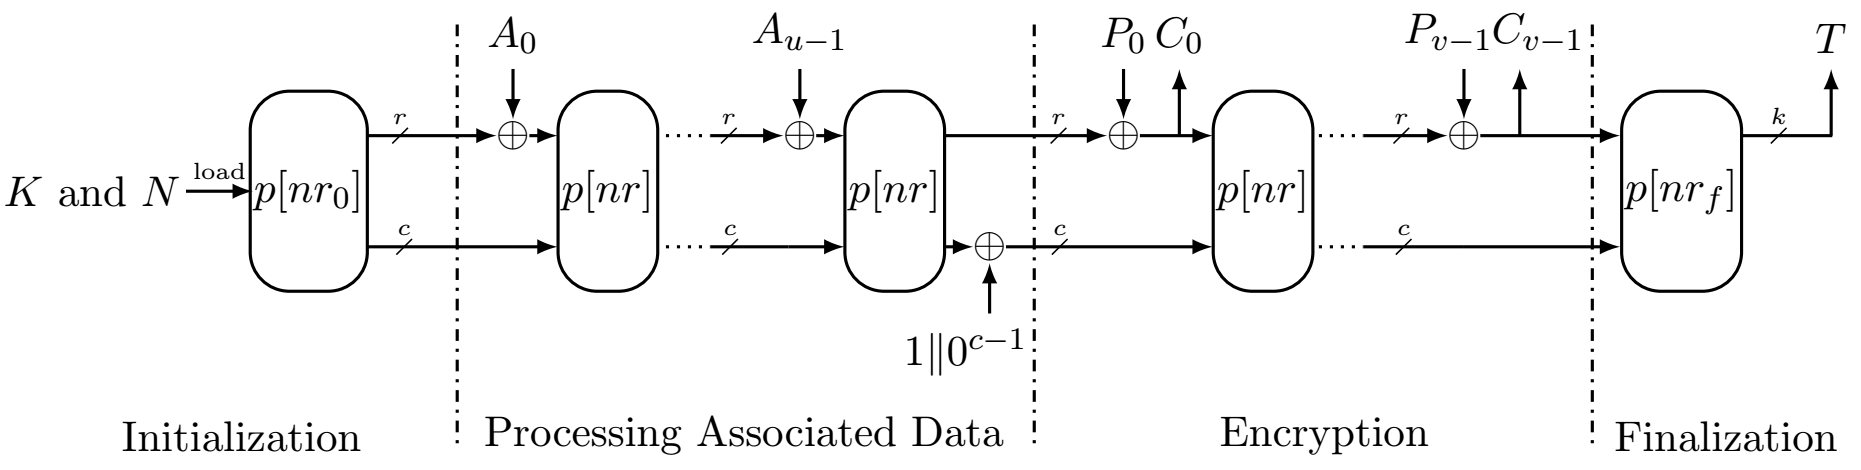
\includegraphics[width=1\textwidth]{fig/mode_aead.PNG}
	\caption{The operation mode of KNOT AEAD} \label{fig:mode_aead}
\end{figure}

\begin{figure}
	\centering
	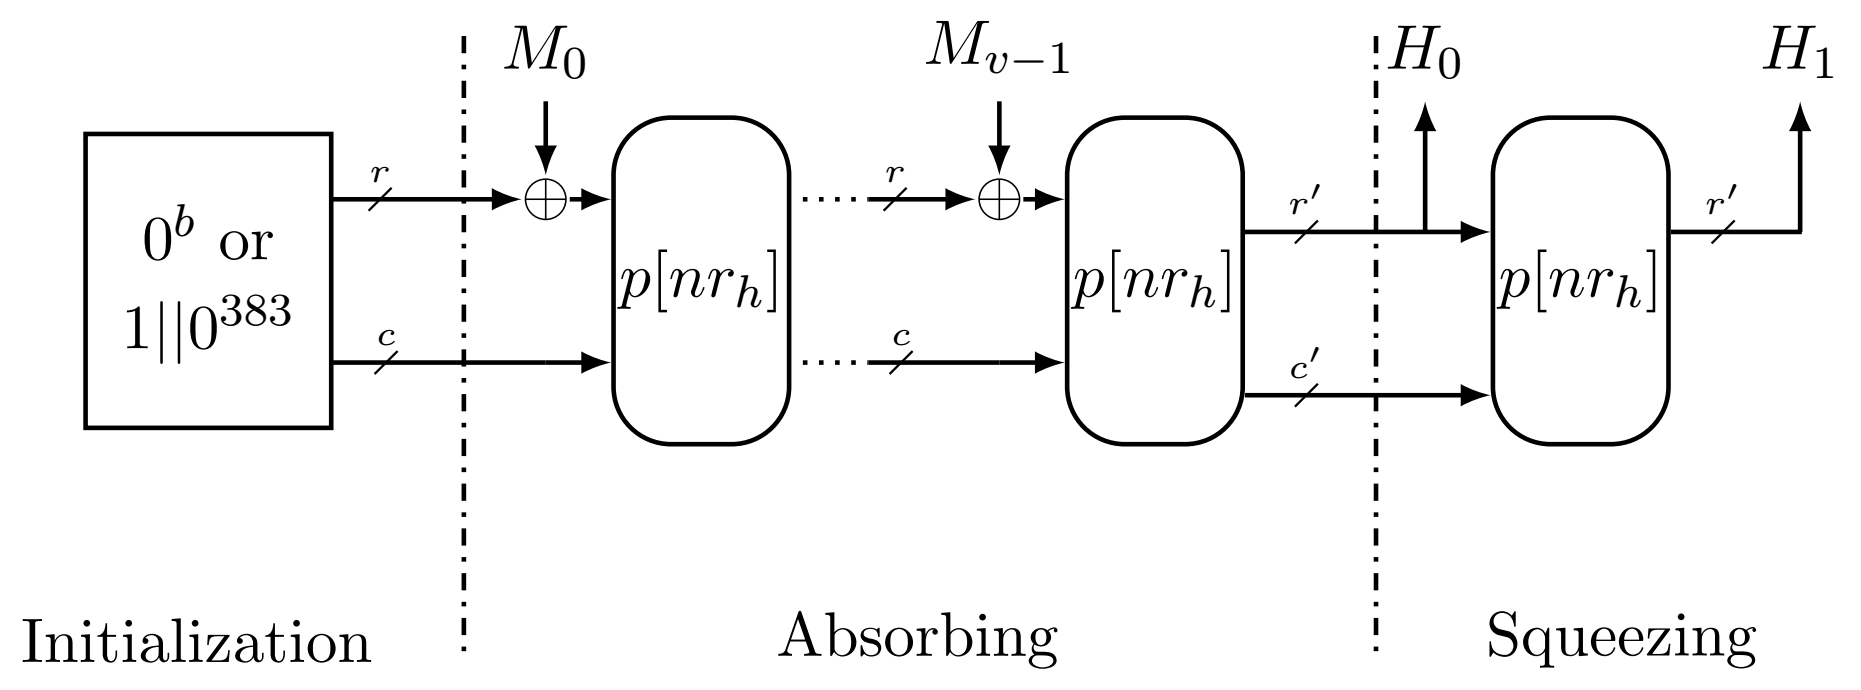
\includegraphics[width=0.7\textwidth]{fig/mode_hash.PNG}
	\caption{The operation mode of KNOT Hash} \label{fig:mode_hash}
\end{figure}

In the original specification document of KNOT, The largest differential probability and linear correlation is given. However, firstly, the differential and linear distinguishers with no restrictions can not be directly uesd to attack the MonkeyDuplex construction. Secondly, the clustering effect is not taken into consideration. Thirdly, because only the rate part and the tag part is visible, differences can be truncated in the capacity part and in the non-tag part. 

For the primary version of KNOT-AEAD, the block, rate, capacity, key and nonce size $b,r,c,k,n$ are $256,64,192,128,128$. For a inner state $S$, we can seperate it by the nonce and key part denoted by $(S_N,S_K),|S_N|=n,|S_K|=k$, by the rate and capacity part denoted by $(S_R,S_C),|S_R|=r,|S_C|=c$, by the tag and non-tag part denoted by $(S_T,S_{nT}),|S_T|=k,|S_{nT}|=b-k$.

For the primary version of KNOT-Hash, the block, rate, capacity and half-tag size $b,r,c,r'$ are $256,32,224,128$. For a inner state $S$, we can seperate it by the rate and capacity part denoted by $(S_R,S_C),|S_R|=r,|S_C|=c$, by the tag and non-tag part denoted by $(S_T,S_{nT}),|S_T|=r',|S_{nT}|=b-r'$.

In the following, we propose differential and linear attacks targeting different phases, each demanding specific restrictions on the distinguishers. The attacks proposed are general for cryptographic schemes based on MonkeyDuplex construction. For each attack, we give the largest differential probability or linear correlation of the longest distinguisher of the primary version of KNOT in Table \ref{tab:knot}.

\begin{itemize}
	\item \textbf{Diff-Init-D} This is a chosen-nonce differential distinguishing attack targeting the initialization phase of KNOT-AEAD. The input difference has the nonce part and key part $\Delta SI=(\Delta SI_N,\Delta SI_K)$. The output difference has the rate part and capacity part $\Delta SO=(\Delta SO_R,\Delta SO_C)$. We restrict that $\Delta SI_K=0$. And $\Delta SO_C$ is truncated. 
	\item \textbf{Linear-Init-KR} This is a known-nonce and known-plaintext linear key recovery attack targeting the initialization phase of KNOT-AEAD. The input mask $\Gamma SI=(\Gamma SI_N,\Gamma SI_K)$ and the output mask $\Gamma SO=(\Gamma SO_R,\Gamma SO_C)$. We restrict that $\Gamma SO_C=0$. Note that if for the best linear distinguisher $\Gamma SI_K\neq 0$, then the attack degrades to a distinguishing one, of which the probability is negligible. 
	\item \textbf{Linear-Enc-D} This is a known-plaintext linear distinguishing attack targeting the encryption phase of KNOT-AEAD. The input mask $\Gamma SI=(\Gamma SI_R,\Gamma SI_C)$ and the output mask $\Gamma SO=(\Gamma SO_R,\Gamma SO_C)$. We restrict that $\Gamma SI_C=0$ and $\Gamma SO_C=0$. 
	\item \textbf{Diff-Enc-F} This is a differential forgery attack targeting the encryption phase of KNOT-AEAD. The input difference $\Delta SI=(\Delta SI_R,\Delta SI_C)$ and the output difference $\Delta SO=(\Delta SO_R,\Delta SO_C)$. We restrict that $\Delta SI_C=0$ and $\Delta SO_C=0$. 
	\item \textbf{Diff-Final-F} This is a differential forgery attack targeting the finalization phase of KNOT-AEAD. The input difference $\Delta SI=(\Delta SI_R,\Delta SI_C)$ and the output difference $\Delta SO=(\Delta SO_T,\Delta SO_{nT})$. We restrictions that $\Delta SI_C=0$. And $\Delta SO_{nT}$ is truncated. 
	\item \textbf{Diff-Col-I} This is a differential collsion attack targeting the absorb phase of KNOT-Hash. The input difference $\Delta SI=(\Delta SI_R,\Delta SI_C)$ and the output difference $\Delta SO=(\Delta SO_R,\Delta SO_C)$. We restrictions that $\Delta SI_C=0$ and $\Delta SO_C=0$. 
	\item \textbf{Diff-Col-II} This is a differential collsion attack targeting the squeezing phase of KNOT-Hash. The input difference $\Delta SI=(\Delta SI_R,\Delta SI_C)$ and the output difference $\Delta SO=(\Delta SO_{T},\Delta SO_{nT})$. We restrict that $\Delta SI_C=0$ and $\Delta SI_{T}=0$. And $\Delta SI_{nT}$ is truncated. 
\end{itemize}

\begin{table}
	\caption{Results on the best differential and linear distinguishers for the primary version of KNOT}\label{tab:knot}
	\centering
	\begin{tabular}{|c|c|c|c|c|c|c|c|}
		\hline
		Attack Model & $r$ & $A$ & $(rb,wb)$ & $-\log_2\bbP$ or $-\log_2\Cor$\\
		\hline
		Diff-Init-D & 14 & 2 & (5,20) & 62.2 \\
		%Linear-Init-KR & 13 & 3 & (3,8) & 30.7*2=61.4 \\
		Linear-Init-KR & 13 & 3 & (3,8) & 31.3 \\%31.28
		%Linear-Enc-D & 12 & 3 & (3,10) & 30.2*2=60.4 \\
		%Linear-Enc-D & 12 & 3 & (3,8) & 30.44 \\
		Linear-Enc-D & 12 & 3 & (3,10) & 30.5 \\%30.52
		Diff-Enc-F & 12 & 2 & (5,20) & 62.4 \\
		Diff-Final-F & 13 & 2 & (5,20) & 61.4 \\
		Diff-Col-I & 12 & 2 & (5,20) & 62.7 \\
		Diff-Col-II & 13 & 2 & (5,20) & 61.4 \\
		\hline
	\end{tabular}
\end{table}

According to Table \ref{tab:knot}, it's suggested that the rounds of the initialization, encryption and finalization phases of KNOT-AEAD should be more than 14, 12 and 13 and the rounds of the absorbing and squeezing phases of KNOT-Hash should be more than 12 and 13. 

\subsection{Comparison with the method of enumerating characteristics}

To verify our results, fixing the input and output differences (masks) as those obtained using our method, we use the MILP method to enumerate characteristics with their differential probabilities (correlation amplitudes) larger than a bound. We respectively check on a 10-round differential and a 10-round linear hull.

For the 10-round difference propagation with input difference $X[32]=0x1, X[49]=0x1$ and output difference $Y[39]=0x1, Y[63]=0x1$, we enumerate its differential characteristics with probabilities between $2^{-56}$ and $2^{-69}$. The number of characteristics grouped by the probabilities are shown in Table \ref{tab:num-diff}. The total weight of a differential w.r.t. the maximum weight of a differential characteristic in it is shown in Figure \ref{fig:plot10-ddt}. We find the line approaches a horizontal one. Thus we believe the probability of the differential is very close to $2^{-53.49}$. Using our method, the number of characteristics grouped by the probabilities are also shown in Table \ref{tab:num-diff}. The probability sum is $2^{-53.53}$, which is very close to that obtained by the MILP method. By Table \ref{tab:num-diff}, the 10-round differential is dominated by characteristics containing iterative sub-characteristics. 

%the differential probability obtained by our method is $2^{-53.7}$ while that obtained by the MILP method is $2^{53.5}$. 

For the 10-round linear propagation with input mask $X[0]=0x1, X[25]=0x1$ and output mask $Y[24]=0x1, Y[41]=0x1$, we enumerate its linear characteristics with correlation amplitudes between $2^{-30}$ and $2^{-40}$. The number of characteristics grouped by the correlation amplitudes are shown in Table \ref{tab:num-linear}. The total weight of a linear hull w.r.t. the maximum weight of a linear characteristic in it is shown in Figure \ref{fig:plot10-lat2}. We find the line approaches a horizontal one. Thus the correlation square sum of the linear hull is very close to $2^{-56.21}$. Using our method, the number of characteristics grouped by the correlation amplitude are also shown in Table \ref{tab:num-linear}. The correlation square sum is $2^{-56.30}$, which is very close to that obtained by the MILP method. By Table \ref{tab:num-linear}, the 10-round linear hull is dominated by characteristics containing iterative sub-characteristics. 
%the linear correlation amplitude obtained by our method is $2^{-26.4}$ while that obtained by the MILP method is $2^{-25.5}$. We list the number of characteristics considered in both methods in Table \ref{tab:num-linear}. Our method underestimates the correlation amplitude for some characteristics with correlation amplitudes no smaller than $2^{34}$ are missing. But it holds that the distinguisher is dominated by iterative characteristics. 

\begin{figure}[htbp]
	\centering
	\caption{The total weight of a differential or linear hull w.r.t. the maximum weight of a characteristic }
	\subfigure[differential]{
	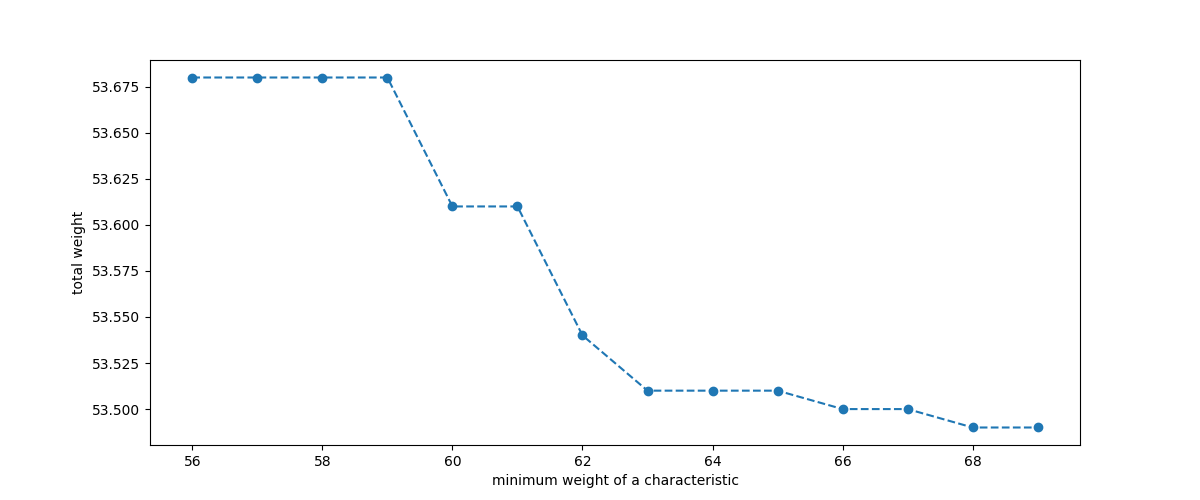
\includegraphics[width=9cm]{fig/plot10_ddt.png}
	\label{fig:plot10-ddt}
	}
	\quad
	\subfigure[linear]{
	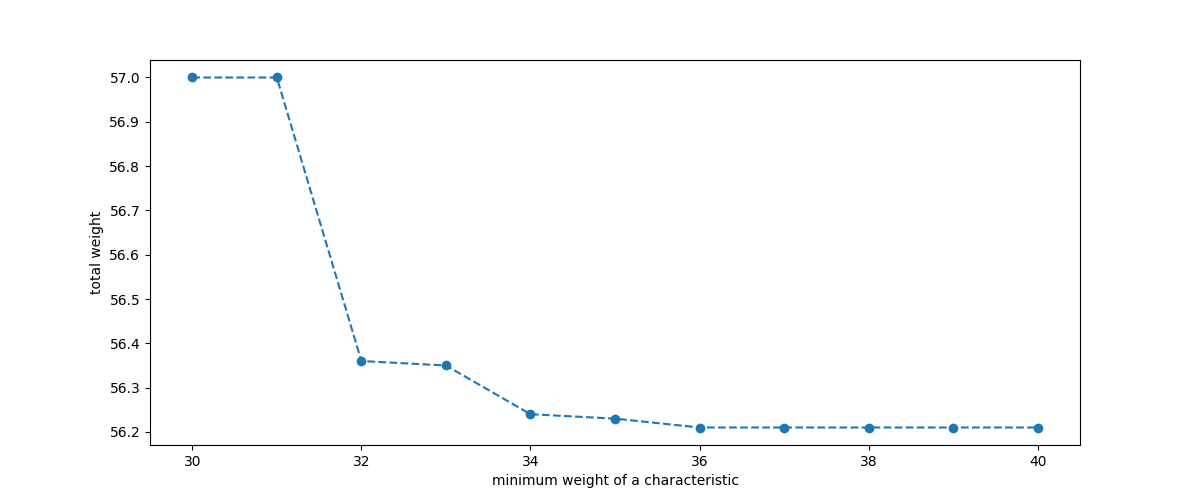
\includegraphics[width=9cm]{fig/plot10_lat2.png}
	\label{fig:plot10-lat2}
	}
	
\end{figure}

\begin{table}
	\caption{Results on the number of characteristics of the 10-round difference propagation grouped by the differential probabilities}\label{tab:num-diff}
	\centering
	\begin{tabular}{|c|c|c|c|c|c|c|c|c|c|c|c|c|c|c|}
		\hline
		$-\log_2|\Prob|$ & 56 & 57 & 58 & 59 & 60 & 61 & 62 & 63 & 64 & 65 & 66 & 67 & 68 & 69 \\
		\hline
		MILP & 5 & 0 & 0 & 0 & 4 & 0 & 17 & 12 & 0 & 12 & 36 & 1 & 38 & 59 \\
		\hline
		ours & 5 & 0 & 0 & 0 & 4 & 0 & 16 & 3 & 0 & 1 & 2 & 0 & 1 & 1\\
		\hline
	\end{tabular}
\end{table}

\begin{table}
	\caption{Results on the number of characteristics of the 10-round linear propagation grouped by the correlation amplitude}\label{tab:num-linear}
	\centering
	\begin{tabular}{|c|c|c|c|c|c|c|c|c|c|c|c|c|c|c|c|}
		\hline
		$-\log_2|\Cor|$ & 30 & 31 & 32 & 33 & 34 & 35 & 36 & 37 & 38 & 39 & 40 & 41 & 42 & 43 & 44\\
		\hline
		MILP & 8 & 0 & 72 & 4 & 264 & 72 & 648 & 364 & 1260 & 1092 & 2196 & - & - & - & - \\
		\hline
		%ours & 8 & 0 & 72 & 4 & 248 & 48 & 392 & 132 & 252 & 148 & 60 & 36 & 12 & 4\\
		ours & 8 & 0 & 64 & 0 & 224 & 8 & 480 & 56 & 736 & 160 & 752 & 216 & 584 & 216 & 224 \\
		\hline
	\end{tabular}
\end{table}



